\documentclass{beamer}
\usepackage{ctex, hyperref}
\usepackage[T1]{fontenc}

% \usepackage[orientation=landscape,size=custom,width=16,height=9,scale=0.4,debug]{beamerposter}
% 修改 slides 比例,

% other packages
\usepackage{latexsym,amsmath,xcolor,multicol,booktabs,calligra}
\usepackage{graphicx,pstricks,listings,stackengine,cite}

\setbeamertemplate{bibliography item}[text]
\bibliographystyle{plain}
% 如果参考文献太多的话,可以像下面这样调整字体:
% \tiny\bibliographystyle{plain}

\author{陈震雄}
\title{Project1: Threads}
\subtitle{PintOS}
\institute{武汉大学}
\date{\today}
\usepackage{College}

% defs
\def\cmd#1{\texttt{\color{red}\footnotesize $\backslash$#1}}
\def\env#1{\texttt{\color{blue}\footnotesize #1}}
\definecolor{deepblue}{rgb}{0,0,0.5}
\definecolor{deepred}{rgb}{0.6,0,0}
\definecolor{deepgreen}{rgb}{0,0.5,0}
\definecolor{halfgray}{gray}{0.55}

\lstset{
    basicstyle=\ttfamily\tiny,
    keywordstyle=\bfseries\color{deepblue},
    emphstyle=\ttfamily\color{deepred},    % Custom highlighting style
    stringstyle=\color{deepgreen},
    numbers=left,
    numberstyle=\tiny\color{halfgray},
    commentstyle=\color{halfgray},
    rulesepcolor=\color{red!20!green!20!blue!20},
    frame=shadowbox,
}

\AtBeginSection[]
{
    \begin{frame}
        \frametitle{Table of Contents}
        \tableofcontents[currentsection]
    \end{frame}
}
\logo{
\includegraphics[height=1cm]{pic/whulogo.pdf}}
\begin{document}
% insert title page---------------------------
\frame{\titlepage}

%insert contents------------------------------
\begin{frame}
    \frametitle{Table of Contents}
    \tableofcontents
\end{frame}
%----------------------
\section{Introduction}
\begin{frame}[fragile]{Introduction}
    In this assignment, we give you a minimally functional thread system. Your job is to \textbf{extend the functionality of this system to gain a better understanding of synchronization problems.}

You will be working primarily in the threads/ directory for this assignment, with some work in the devices/ directory on the side.

Compilation should be done in the threads/ directory.
\end{frame}
%------------------
\section{Task 1: Alarm Clock}
\begin{frame}[fragile]{Exercise 1.1}
Reimplement timer\_sleep(), defined in devices/timer.c.

Although a working implementation is provided, it "busy waits," that is, it spins in a loop checking the current time and calling thread\_yield() until enough time has gone by.

Reimplement it to avoid busy waiting.
\end{frame}
\begin{frame}[fragile]{The original implement of timer\_sleep}
begin->check not OK->intr disable->take out->input ready list->intr on->...->check OK->exit
\begin{lstlisting}[language=C]
void
timer_sleep (int64_t ticks) 
{
  int64_t start = timer_ticks ();

  ASSERT (intr_get_level () == INTR_ON);
  while (timer_elapsed (start) < ticks) 
    thread_yield ();
}
\end{lstlisting}
\end{frame}
\begin{frame}[fragile]{Reimplement of timer\_sleep}
begin->block->put into sleep list->check block threads (in timer interrupt)->...->OK
\begin{lstlisting}[language=C]
// timer.c
static struct list sleep_list;
void timer_init (void) {
    ...
    list_init (&sleep_list);
}
void timer_sleep (int64_t ticks) {
  if (ticks <= 0)
    return;
  ASSERT (intr_get_level () == INTR_ON);
  struct thread * t = thread_current ();
  enum intr_level old_level = intr_disable ();
  t->ticks_blocked = timer_ticks () + ticks;
  list_insert_ordered (&sleep_list, &t->elem, thread_less_ticks_blocked, NULL);
  thread_block ();
  intr_set_level (old_level);
}
// thread.c
static void init_thread (struct thread *t, const char *name, int priority) {
    ...
    t->ticks_blocked = 0;
    ...
}
\end{lstlisting}
\end{frame}
\begin{frame}[fragile]{Reimplement of timer\_sleep}
begin->block->put into sleep list->check block threads (in timer interrupt)->...->OK
\begin{lstlisting}[language=C]
// timer.c
static void timer_interrupt (struct intr_frame *args UNUSED) {
  struct list_elem* e;
  struct thread* t;
  ticks++;
  thread_tick ();
  while (!list_empty (&sleep_list))
  {
    e = list_front (&sleep_list);
    t = list_entry (e, struct thread, elem);
    if (t->ticks_blocked > timer_ticks ())
      break;
    list_remove (e);
    thread_unblock (t);
  }
}
// thread.c
bool thread_less_ticks_blocked (const struct list_elem *a, 
const struct list_elem *b, void *aux UNUSED)
{
  return list_entry (a, struct thread, elem)->ticks_blocked 
  < list_entry (b, struct thread, elem)->ticks_blocked;
}
\end{lstlisting}
\end{frame}
%----
\section{Task 2: Priority Scheduling}
\subsection{Exercise 2.1}
\begin{frame}[fragile]{Exercise 2.1}
\textbf{Implement priority scheduling in Pintos.}

When a thread is added to the ready list that has a higher priority than the currently running thread, the current thread should \textbf{immediately yield} the processor to the new thread.

Similarly, when threads are waiting for a lock, semaphore, or condition variable, \textbf{the highest priority waiting thread should be awakened first.}

A thread may raise or lower its own priority at any time, but \textbf{lowering its priority such that it no longer has the highest priority must cause it to immediately yield the CPU.}
\end{frame}
\subsection{Exercise 2.2}
\begin{frame}[fragile]{Exercise 2.2.1}
    \textbf{Implement priority donation.
You will need to account for all different situations in which priority donation is required.}

You must implement priority donation \textbf{for locks.} You need \textbf{not} implement priority donation for the other Pintos synchronization constructs.

You do need to \textbf{implement priority scheduling in all cases.}

Be sure to \textbf{handle multiple donations}, in which multiple priorities are donated to a single thread.
\end{frame}

\begin{frame}[fragile]{Exercise 2.2.2}
    \textbf{Support nested priority donation}:

if H is waiting on a lock that M holds and M is waiting on a lock that L holds, then both M and L should be boosted to H's priority.

If necessary, you may impose \textbf{a reasonable limit} on depth of nested priority donation, such as 8 levels.
\end{frame}
\subsection{Exercise 2.3}
\begin{frame}[fragile]{}
    \textbf{Implement the following functions that allow a thread to examine and modify its own priority.}

Skeletons for these functions are provided in \textbf{threads/thread.c.}

Function: void thread\_set\_priority (int new\_priority)

Function: int thread\_get\_priority (void)
\end{frame}
%----
\subsection{Solution}
\begin{frame}[fragile]{Part1: Basic}
\begin{lstlisting}[language=C]
// thread.c
static void init_thread (struct thread *t, const char *name, int priority) {
  ...
  list_insert_ordered (&all_list, &t->allelem, thread_greater_fun, NULL);
  ...
}
void thread_unblock (struct thread *t) {
  ...
  list_insert_ordered (&ready_list, &t->elem, thread_greater_fun, NULL);
  ...
}
void thread_yield (void) {
    ...
    list_insert_ordered (&ready_list, &cur->elem, thread_greater_fun, NULL);
    ...
}
tid_t thread_create (const char *name, int priority, thread_func *function, 
void *aux) {
  ...
  if (thread_current ()->priority < priority) {
    thread_yield();
  }
  ...
}
\end{lstlisting}
\end{frame}
\begin{frame}[fragile]{Part1 Basic}
\begin{lstlisting}[language=C]
/** Greater fuc for thread. */
bool thread_greater_fun (const struct list_elem
*a, const struct list_elem *b, void *aux UNUSED)
{
  return list_entry (a, struct thread, elem)->priority >
  list_entry (b, struct thread, elem)->priority;
}
/** Sets the current thread's priority to NEW_PRIORITY. */
void
thread_set_priority (int new_priority) 
{
  thread_current ()->priority = new_priority;
  thread_yield();
}
\end{lstlisting}
\end{frame}
\begin{frame}[fragile]{Part2 Data struct}
\begin{lstlisting}[language=C]
// thread.h
struct thread {
    ...
    int64_t ticks_blocked;              /**< Blocked ticks. */
    int base_priority;                  /**< Base priotiry. */
    struct list locks_holding;          /**< Holding locks. */
    struct lock *lock_waiting;          /**< Waiting lock */
    ...
}
// synch.h
struct lock {
    ...
    struct list_elem elem;      /**< Insert into thread's lock_list by this. */
    int max_priority;           /**< Accquiring thread max priority. */
  };
// thread.c
static void init_thread (struct thread *t, const char *name, int priority) {
  ...
  t->ticks_blocked = 0;
  t->base_priority = priority;
  list_init (&t->locks_holding);
  t->lock_waiting = NULL;
  ...
}
\end{lstlisting}
\end{frame}
%------
\begin{frame}[fragile]{Part2 acquire lock}
\begin{columns}
\begin{column}{0.5\textwidth}
\begin{lstlisting}[language=C]
// synch.c
void lock_acquire (struct lock *lock)
{
  struct thread *t = thread_current ();
  struct lock* l;
  enum intr_level old_level;

  ASSERT (lock != NULL);
  ASSERT (!intr_context ());
  ASSERT (!lock_held_by_current_thread 
  (lock));

  /* Lock locks, donate priority if OK. 
  nest*/
  if (lock->holder != NULL && 
  !thread_mlfqs)
  {
    t->lock_waiting = lock;
    l = lock;
    while (l && t->priority > 
    l->max_priority)
    {
      l->max_priority = t->priority;
      thread_donate_priority(l->holder);
      l = l->holder->lock_waiting;
    }
  }

\end{lstlisting}
\end{column}
\begin{column}{0.5\textwidth}
\begin{lstlisting}[language=C]
  /* Get lock. */
  sema_down (&lock->semaphore);
  /* Ensure lock's owner change correctly.
     (Get lock correctly.) */
  old_level = intr_disable ();    
  t = thread_current ();
  /* Change lock max priority. */
  if (!thread_mlfqs)
  {
    t->lock_waiting = NULL;
    lock->max_priority = t->priority;
  /* Hold lock. */  
    thread_hold_the_lock (lock);
  }
  lock->holder = thread_current ();
  intr_set_level (old_level);
}
/* lock greater_priority function */
bool lock_greater_priority (const struct 
list_elem *a, const struct list_elem *b, 
void *aux UNUSED)
{
  return list_entry (a, struct lock, elem)
  ->max_priority >
  list_entry (b, struct lock, elem)
  ->max_priority;
}
\end{lstlisting}
\end{column}
\end{columns}
\end{frame}
\begin{frame}[fragile]{Part2 acquire lock}
\begin{columns}
\begin{column}{0.5\textwidth}
\begin{lstlisting}[language=C]
void
thread_update_priority (struct thread *t)
{
  enum intr_level old_level = 
  intr_disable ();
  int max_priority = t->base_priority;
  int lock_priority;

  if (!list_empty (&t->locks_holding))
  {
    list_sort (&t->locks_holding, 
    lock_greater_priority, NULL);
    lock_priority = list_entry (
    list_front (&t->locks_holding),
    struct lock, elem)->max_priority;
    if (lock_priority > max_priority)
      max_priority = lock_priority;
  }

  t->priority = max_priority;
  intr_set_level (old_level);
}
/** Donate priority. */
void
thread_donate_priority (struct thread *t)
{
\end{lstlisting}
\end{column}
\begin{column}{0.5\textwidth}
\begin{lstlisting}[language=C]
  enum intr_level old_level = 
  intr_disable ();
  thread_update_priority (t);
  if (t->status == THREAD_READY)
  {
    list_remove (&t->elem);
    list_insert_ordered (&ready_list,
    &t->elem,
    thread_greater_priority, NULL);
  }
  intr_set_level (old_level);
}

/** Thread hold lock. */
void 
thread_hold_the_lock (struct lock* lock)
{
  enum intr_level old_level = 
  intr_disable ();
  list_insert_ordered (&thread_current ()
  ->locks_holding, 
  &lock->elem, 
  lock_greater_priority, NULL);
  intr_set_level (old_level);
}
\end{lstlisting}
\end{column}
\end{columns}
\end{frame}
\begin{frame}[fragile]{Part2 lock release}
\begin{lstlisting}[language=C]
// thread.c
void
lock_release (struct lock *lock) 
{
  if (!thread_mlfqs)
    thread_remove_lock(lock);
  ASSERT (lock != NULL);
  ASSERT (lock_held_by_current_thread (lock));

  lock->holder = NULL;
  sema_up (&lock->semaphore);   /**< Schedule in sema_up. */
}

/** Thread remove lock. */
void
thread_remove_lock (struct lock *lock)
{
  enum intr_level old_level = intr_disable ();
  list_remove (&lock->elem);
  thread_update_priority (thread_current ());
  intr_set_level (old_level);
}
\end{lstlisting}
\end{frame}
\begin{frame}[fragile]{Part3 Sema}
Priority queue. When sema up, we should \textbf{SORT IT!}
\begin{lstlisting}[language=C]
// synch.c
void sema_down (struct semaphore *sema) {
    ...
    list_insert_ordered (&sema->waiters, 
    &thread_current ()->elem, thread_greater_priority, NULL);
    ...
}
void
sema_up (struct semaphore *sema) 
{
  enum intr_level old_level;

  ASSERT (sema != NULL);

  old_level = intr_disable ();
  if (!list_empty (&sema->waiters)) 
  {
    list_sort (&sema->waiters, thread_greater_priority, NULL);
    thread_unblock (list_entry (list_pop_front (&sema->waiters),
                                struct thread, elem));
  }
  sema->value++;
  thread_yield ();
  intr_set_level (old_level);
}
\end{lstlisting}
\end{frame}
\begin{frame}[fragile]{Cond}
Priority queue too.
\begin{lstlisting}[language=C]
void
cond_signal (struct condition *cond, struct lock *lock UNUSED) 
{
  ASSERT (cond != NULL);
  ASSERT (lock != NULL);
  ASSERT (!intr_context ());
  ASSERT (lock_held_by_current_thread (lock));

  if (!list_empty (&cond->waiters)) 
  list_sort (&cond->waiters, cond_sema_greater_priority, NULL);
  sema_up (&list_entry (list_pop_front (&cond->waiters),
                       struct semaphore_elem, elem)->semaphore);
}

/** cond sema greater function. */
bool 
cond_sema_greater_priority (const struct list_elem *a, const struct list_elem *b, 
void *aux UNUSED)
{
  struct semaphore_elem *sa = list_entry (a, struct semaphore_elem, elem);
  struct semaphore_elem *sb = list_entry (b, struct semaphore_elem, elem);
  return list_entry(list_front(&sa->semaphore.waiters), struct thread, elem)->priority > list_entry(list_front(&sb->semaphore.waiters),
  struct thread, elem)->priority;
}
\end{lstlisting}
\end{frame}
%-------
\section{Task3: Advanced Scheduler}
\begin{frame}[fragile]{Exercise 3.1}
    \textbf{Implement a multilevel feedback queue scheduler} similar to the 4.4BSD scheduler to reduce the average response time for running jobs on your system.

See section 4.4BSD Scheduler, for detailed requirements.
\end{frame}
%------
\begin{frame}{Fixed-Point Arithmetic Operations}
\small
\begin{table}
\begin{tabular}{ll}
\toprule
\textbf{Operation} & \textbf{Expression} \\
\midrule
Convert $n$ to fixed point & $n \cdot f$ \\
Convert $x$ to integer (rounding toward zero) & $x / f$ \\
Convert $x$ to integer (rounding to nearest) & 
    $\begin{cases} 
    (x + f / 2) / f & \text{if } x \geq 0 \\ 
    (x - f / 2) / f & \text{if } x \leq 0 
    \end{cases}$ \\
Add $x$ and $y$ & $x + y$ \\
Subtract $y$ from $x$ & $x - y$ \\
Add $x$ and $n$ & $x + n \cdot f$ \\
Subtract $n$ from $x$ & $x - n \cdot f$ \\
Multiply $x$ by $y$ & $((\text{int64\_t}) \, x) \cdot y / f$ \\
Multiply $x$ by $n$ & $x \cdot n$ \\
Divide $x$ by $y$ & $((\text{int64\_t}) \, x) \cdot f / y$ \\
Divide $x$ by $n$ & $x / n$ \\
\bottomrule
\end{tabular}
\end{table}
\end{frame}
%------
\begin{frame}[fragile]{Part1 Fixed point}
\begin{lstlisting}[language=C]
// fixed-point.h
#ifndef __THREAD_FIXED_POINT_H
#define __THREAD_FIXED_POINT_H
/* Basic definitions of fixed point. */
typedef int fixed_t;
/* 16 LSB used for fractional part. */
#define FP_SHIFT_AMOUNT 14
/* Convert a value to fixed-point value. */
#define FP_CONST(A) ((fixed_t)(A << FP_SHIFT_AMOUNT))
/* Get integer part of a fixed-point value. */
#define FP_INT_PART(A) (A >> FP_SHIFT_AMOUNT)
/* Get rounded integer of a fixed-point value. */
#define FP_ROUND(A) (A >= 0 ? ((A + (1 << (FP_SHIFT_AMOUNT - 1))) >> FP_SHIFT_AMOUNT)\
        : ((A - (1 << (FP_SHIFT_AMOUNT - 1))) >> FP_SHIFT_AMOUNT))
/* Add two fixed-point value. */
#define FP_ADD(A,B) (A + B)
/* Substract two fixed-point value. */
#define FP_SUB(A,B) (A - B)
/* Add a fixed-point value A and an int value B. */
#define FP_ADD_MIX(A,B) (A + (B << FP_SHIFT_AMOUNT))
/* Substract an int value B from a fixed-point value A */
#define FP_SUB_MIX(A,B) (A - (B << FP_SHIFT_AMOUNT))
#define FP_MULT(A,B) ((fixed_t)(((int64_t) A) * B >> FP_SHIFT_AMOUNT))
#define FP_MULT_MIX(A,B) (A * B)
#define FP_DIV(A,B) ((fixed_t)((((int64_t) A) << FP_SHIFT_AMOUNT) / B))
#define FP_DIV_MIX(A,B) (A / B)
#endif /* thread/fixed_point.h */
\end{lstlisting}
\end{frame}
%-------
\begin{frame}[fragile]{Part2: Nice, loadavg, current cpu}
\begin{lstlisting}[language=C]
// thread.h
struct thread {
    ...
    int nice;                           /* Niceness. */
    fixed_t recent_cpu;                 /* Recent CPU. */
    ...
}
// thread.c
fixed_t load_avg;               /**< Load average. */
void thread_start (void) {
    ...
    load_avg = FP_CONST (0);
    ...
}
static void
init_thread (struct thread *t, const char *name, int priority)
{
    ...
    t->nice = 0;
  if (name=="main")
    t->recent_cpu = FP_CONST (0);
  else
    t->recent_cpu = thread_current ()->recent_cpu;
    ....
}
\end{lstlisting}
\end{frame}
\begin{frame}[fragile]{Nice}
\begin{lstlisting}[language=C]
void
thread_set_nice (int nice UNUSED) 
{
  /* Not yet implemented. */
  thread_current ()->nice = nice;
  thread_mlfqs_update_priority (thread_current ());
  thread_yield ();
}
/** Returns the current thread's nice value. */
int
thread_get_nice (void) 
{
  /* Not yet implemented. */
  return thread_current ()->nice;
}
\end{lstlisting}
\end{frame}
\begin{frame}[fragile]{Load avg and recent cpu}
\begin{lstlisting}[language=C]
/** Returns 100 times the system load average. */
int
thread_get_load_avg (void) 
{
  /* Not yet implemented. */
  return FP_ROUND (FP_MULT_MIX (load_avg, 100));
}
/** Returns 100 times the current thread's recent_cpu value. */
int
thread_get_recent_cpu (void) 
{
  /* Not yet implemented. */
  return FP_ROUND (FP_MULT_MIX (thread_current ()->recent_cpu, 100));
}
\end{lstlisting}
\end{frame}
%-------
\begin{frame}[fragile]{Load avg and recent cpu}
\begin{columns}
\begin{column}{0.5\textwidth}
\begin{lstlisting}[language=C]
// thread.c
void
thread_mlfqs_increase_recent_cpu_by_one 
(void) {
  ASSERT (thread_mlfqs);
  ASSERT (intr_context ());
  struct thread *current_thread =
  thread_current ();
  if (current_thread == idle_thread)
    return;
  current_thread->recent_cpu = 
  FP_ADD_MIX (current_thread->recent_cpu, 1);
}
void thread_mlfqs_update_priority 
(struct thread *t) {
  if (t == idle_thread)
    return;
  ASSERT (thread_mlfqs);
  ASSERT (t != idle_thread);
  t->priority = FP_INT_PART (FP_SUB_MIX 
  (FP_SUB (FP_CONST (PRI_MAX), 
  FP_DIV_MIX (t->recent_cpu, 4)), 
  2 * t->nice));
  t->priority = t->priority < PRI_MIN ?
  PRI_MIN : t->priority;
  t->priority = t->priority > PRI_MAX ?
  PRI_MAX : t->priority;
}
\end{lstlisting}
\end{column}
\begin{column}{0.5\textwidth}
\begin{lstlisting}[language=C]
void
thread_mlfqs_update_load_avg_and_recent_cpu
(void) {
  ASSERT (thread_mlfqs);
  ASSERT (intr_context ());
  size_t ready_threads = list_size 
  (&ready_list);
  if (thread_current () != idle_thread)
    ready_threads++;
  load_avg = FP_ADD (FP_DIV_MIX 
  (FP_MULT_MIX (load_avg, 59), 60), 
  FP_DIV_MIX (FP_CONST (ready_threads), 60));
  struct thread *t;
  struct list_elem *e=list_begin (&all_list);
  for (; e != list_end (&all_list); 
  e = list_next (e)) {
    t = list_entry(e, struct thread, 
    allelem);
    if (t != idle_thread) {
      t->recent_cpu = FP_ADD_MIX 
      (FP_MULT (FP_DIV (FP_MULT_MIX
      (load_avg, 2), FP_ADD_MIX 
      (FP_MULT_MIX (load_avg, 2), 1)), 
      t->recent_cpu), t->nice);
      thread_mlfqs_update_priority (t);
    }
  }
}
\end{lstlisting}
\end{column}
\end{columns}
\end{frame}
\begin{frame}[fragile]{Timer interrupt}
It's time to call them.
\begin{lstlisting}[language=C]
static void
timer_interrupt (struct intr_frame *args UNUSED)
{
    ...
      /* MLFQS check. */
  if (thread_mlfqs)
  {
    thread_mlfqs_increase_recent_cpu_by_one ();
    if (ticks % TIMER_FREQ == 0)
      thread_mlfqs_update_load_avg_and_recent_cpu ();
    else if (ticks % 4 == 0)
      thread_mlfqs_update_priority (thread_current ());
  }
}
\end{lstlisting}
\end{frame}
\begin{frame}[fragile]{Some terrible bugs}
\small
    \begin{figure}
        \centering
        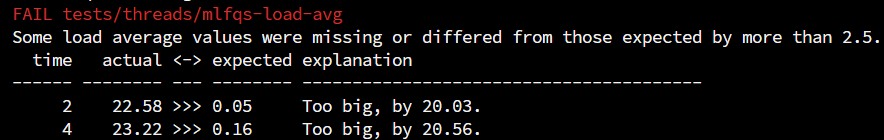
\includegraphics[width=0.8\linewidth]{pic/bugs.png}    
    \end{figure}
Q: Some scheduler tests fail and I don't understand why. Help!
A: Consider how much work your implementation does in the timer interrupt. If the timer interrupt handler takes too long, then it will take away most of a timer tick from the thread that the timer interrupt preempted. When it returns control to that thread, it therefore won't get to do much work before the next timer interrupt arrives. That thread will therefore get blamed for a lot more CPU time than it actually got a chance to use. This raises the interrupted thread's recent CPU count, thereby lowering its priority. It can cause scheduling decisions to change. It also raises the load average.
\end{frame}
\begin{frame}[fragile]{Result}
    \begin{figure}
        \centering
        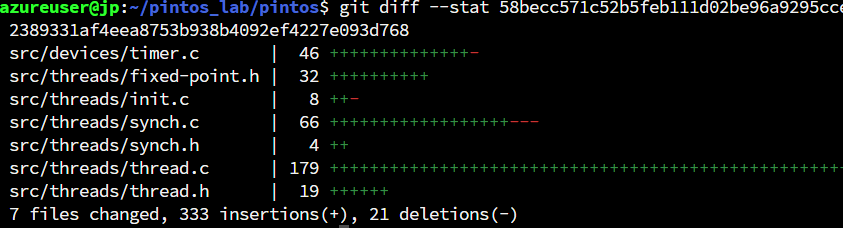
\includegraphics[width=0.8\linewidth]{pic/result1.png}
        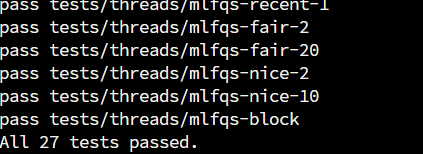
\includegraphics[width=0.8\linewidth]{pic/result2.png}
    \end{figure}
\end{frame}
\begin{frame}{The End}
    \centering
    \vfill
    \Huge
    \textbf{Thank you!}
    \vfill
    \normalsize
    Any questions?
    \vfill
\end{frame}
\end{document}
